\documentclass{beamer}

\usepackage{ucs}
\usepackage[utf8x]{inputenc}
\usepackage[T1]{fontenc}
\usepackage[english]{babel}
\usepackage{epstopdf}
\usepackage{graphicx}

%\usepackage{multirow}%	multirow
%\usepackage[retainorgcmds]{IEEEtrantools}%	IEEEeqnarray
%\usepackage{mathabx}%	convolution symbol
\usepackage{relsize}%	relative font sizes
%\usepackage{listings}
%\usepackage{graphicx}
\usepackage{multicol}
\usepackage{listings}
\usepackage{color}

\lstset{
	language=C++,
	basicstyle=\ttfamily\footnotesize,
	showspaces=false,
	showtabs=false,
	tabsize=3,
	captionpos=b,
	breaklines=true,
	breakatwhitespace=true
}


%	presentation info
\title{Parallel Radix Sort}
\subtitle{OpenMP and MPI Analysis}
\author{Miguel Palhas, pg19808@alunos.uminho.pt \\
	\footnotesize{\url{www.github.com/naps62/parallel-sort}}}
\institute[19808]{
	University of Minho\\
	Department of Informatics
}
\date{Braga, May 2012}


%	beamer options
\usetheme{CambridgeUS}


\begin{document}%	begin presentation

\maketitle

\begin{frame}
	\frametitle{Index}
	\tableofcontents
\end{frame}

\section{Radix Sort}

\begin{frame}
	\frametitle{Sequential Radix Sort}

	\begin{itemize}\itemsep=10pt
		\item Non-comparative sorting algorithm
		\item Works on integer or string keys
		\item Sort is done based on digits
		\item For each digit, set is iterated once
		\begin{itemize}
			\item[-] Complexity $O(k \cdot N)$, where $k$ is number of digits of the largest key
		\end{itemize}

		\item Two versions
			\begin{itemize}
				\item[-] \textbf{Least Significant Digit}: Iterative, easy to implement, hard to parallelize
				\item[-] \textbf{Most Significant Digit}: Recursive, trivial to parallelize, but no load balance
				\item[-] This project considers only the LSD version
			\end{itemize}
	\end{itemize}
\end{frame}

\begin{frame}
   \frametitle{Sequential Radix Sort - Example}

	Initial array:
	\begin{lstlisting}^^J
		arr = [170, 45, 75, 90, 802, 24, 2, 66]^^J
	\end{lstlisting}

	First iteration (sort by first digit)
	\begin{lstlisting}^^J
		0: [170, 90],^^J
		2: [802, 2],^^J
		4: [24],^^J
		5: [45, 75],^^J
		6: [66]^^J
	\end{lstlisting}

	Result after first iteration:
	\begin{lstlisting}^^J
		arr = [170, 90, 802, 2, 24, 45, 75, 66]^^J
	\end{lstlisting}
	
\end{frame}

\section{Sequential}

\begin{frame}
	\frametitle{Sequential Radix Sort - Implementation}

	\begin{itemize}\itemsep=10pt
		\item Bitwise operators, and base 2 digits are used, allowing better performance.\\

		\item Amount of bits per digit ($g$) influences total number of buckets ($B = 2^g$)
		
		\begin{description}\itemsep=8pt
			\item[small $g$] Less buckets, but more iterations
			\item[big $g$] More buckets and less iterations, but more fragmentation and memory overhead
		\end{description}

	\end{itemize}

\end{frame}
   % radix
\section{OpenMP}

\begin{frame}
	\frametitle{OpenMP Implementation}

	Each iteration now has three steps

\begin{enumerate}\itemsep=15pt
		\item Bucket fill
		\begin{itemize}
			\item[-] With $P$ threads, each thread handles P/B buckets
			\item[-] Each thread iterates entire array, but tasks are not homogeneous
		\end{itemize}

		\item Master thread computes offset for each bucket

		\item Each thread copies keys on buckets to global array
	\end{enumerate}
\end{frame}
     % omp implementation
\section{MPI}

\begin{frame}
	\frametitle{Initial MPI Implementation}

	\begin{itemize}
		\item[] Each process starts with an initial partition of the array

		\item[] Like the OpenMP version, each bucket is assigned to a process
	\end{itemize}


	\begin{enumerate}\itemsep=15pt
		\item Local Bucket fill

		\item \emph{1-to-all} transpose operation
		\begin{itemize}
			\item Bucket sizes are sent to the processes that they are assigned to
		\end{itemize}

		\item Communication
		\begin{itemize}
			\item Send/Receive local keys to where they belong
		\end{itemize}

	\end{enumerate}

	After each iteration, load balance changes completely
\end{frame}
     % mpi implementation
\subsection{Load Balance}

\begin{frame}
	\frametitle{MPI Implementation - Load Balance}

	\begin{minipage}[b]{0.45\linewidth}
		\begin{figure}[!htpb]
			\begin{center}
				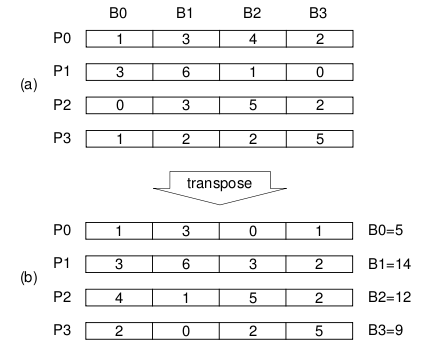
\includegraphics[width=\textwidth]{images/mpi}
			\end{center}
		\end{figure}
	\end{minipage}
	\hspace{0.5cm}
	\begin{minipage}[b]{0.45\linewidth}
		\begin{figure}[!htpb]
			\begin{center}
				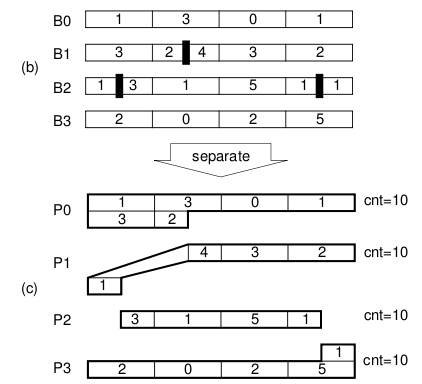
\includegraphics[width=\textwidth]{images/mpi_bal}
			\end{center}
		\end{figure}
	\end{minipage}
\end{frame}
 % mpi load balance
\section{Results}

\begin{frame}
	\frametitle{Testing Methodology}

\begin{itemize}\itemsep=10pt
		\item Tested on SeARCH nodes 6x1 (12x X5650 @ 2.67GHz)
		\item $2^{27}$ keys on biggest test case
		\item Tested with bits per digit ($g$) set to 2, 4 and 8
		\item OpenMP tested for 4, 8 and 16 threads
		\item MPI tested for:
		\begin{itemize}
			\item 1 node, 4 and 8 processes
			\item 2 nodes, 16 and 32 processes
			\item 3 nodes, 64 processes
		\end{itemize}

		\item Also tested on nodes 511, 311 and 101
	\end{itemize}

\end{frame}
  % testing methodology
\begin{frame}
	TODO resultados aqui
\end{frame}
 % test results
\section{Conclusion}

\begin{frame}
	\frametitle{Conclusion}

\begin{itemize}\itemsep=10pt
		\item Radix sort is completely memory bound
		\begin{itemize}
			\item[-] Easily confirmed by observing the C++ code
			\item[-] OpenMP not homogeneous, gives bad results
		\end{itemize}


		\item MPI shows speedups for larger input sizes, but nothing amazing
		\begin{itemize}
			\item[-] Implementation problems
			\item[-] Source paper \footnote{\emph{``Load Balanced Parallel Radix Sort''}, Andrew Sohn and Yuetsu Kodama} claims 40-fold speedups with 64 processors
		\end{itemize}

	\item Load Balanced strategy proved useful for bigger inputs
		\begin{itemize}
			\item[-] But technical problems prevented further analysis
		\end{itemize}

	\end{itemize}

\end{frame}
 % conclusion


\section{Questions}
\begin{frame}
	\titlepage
	\begin{center}
		\Huge\bfseries
		- ? -
	\end{center}
\end{frame}

\end{document}%	end presentation
